\chapter{Implementation}

%The implementation should look at any issues you encountered as you tried to implement your design. During the work, you might have found that elements of your design were unnecessary or overly complex; perhaps third party libraries were available that simplified some of the functions that you intended to implement. If things were easier in some areas, then how did you adapt your project to take account of your findings?

%It is more likely that things were more complex than you first thought. In particular, were there any problems or difficulties that you found during implementation that you had to address? Did such problems simply delay you or were they more significant? 

%You can conclude this section by reviewing the end of the implementation stage against the planned requirements. 

\section{Database}
\textbf{NOTES: - DELETE THIS -}
\begin{itemize}
	\item Nodes and Ways downloaded from OpenStreetMap\cite{OSM}, and stored in a \textit{.osm} file. Size of downloadable area restricted.
	\item All data read by an XML-reader made by Vogella \cite{Vogella-XML}, and stored in two separate Arrays for Nodes and Ways (The type: Relations is not stored). Data filtered afterwards in order to reduce memory-requirements, and to speed up route-planning.
\end{itemize}



\section{Search}
\textbf{NOTES: - DELETE THIS -}
\begin{itemize}
	\item Is this where I describe my algorithms, or do I do that in chapter 2?
	\item A Star, Breadth First Search, Depth First Search, Greedy Best First Search.
	\item PQ did not reorder after the values of its contents changed (after being sorted).
	\item PQ and expansion list not cleared between runs. Used old routes. (Touch on how this can be a good thing if done properly; time/space complexity).
	\item Only tower Nodes used for navigation. Very useful as some ways can have >100 Nodes, but far fewer connections to other Ways.
	\item Three enums: 'Permitted tags', 'Disallowed tags', and 'Area tags' dictate the way in which Nodes are expanded, discarded and handled afterwards.
\end{itemize}

\begin{figure}
	\centering
	\caption[Sup-optimal path due to bad data]{This image shows what can happen to a route if the algorithms are working with bad data. The path between the start and goal positions is not included in the .osm-file, so the search-algorithms were forced to find a much longer route.}
	\label{fig:badDataBadPath}
	\frame{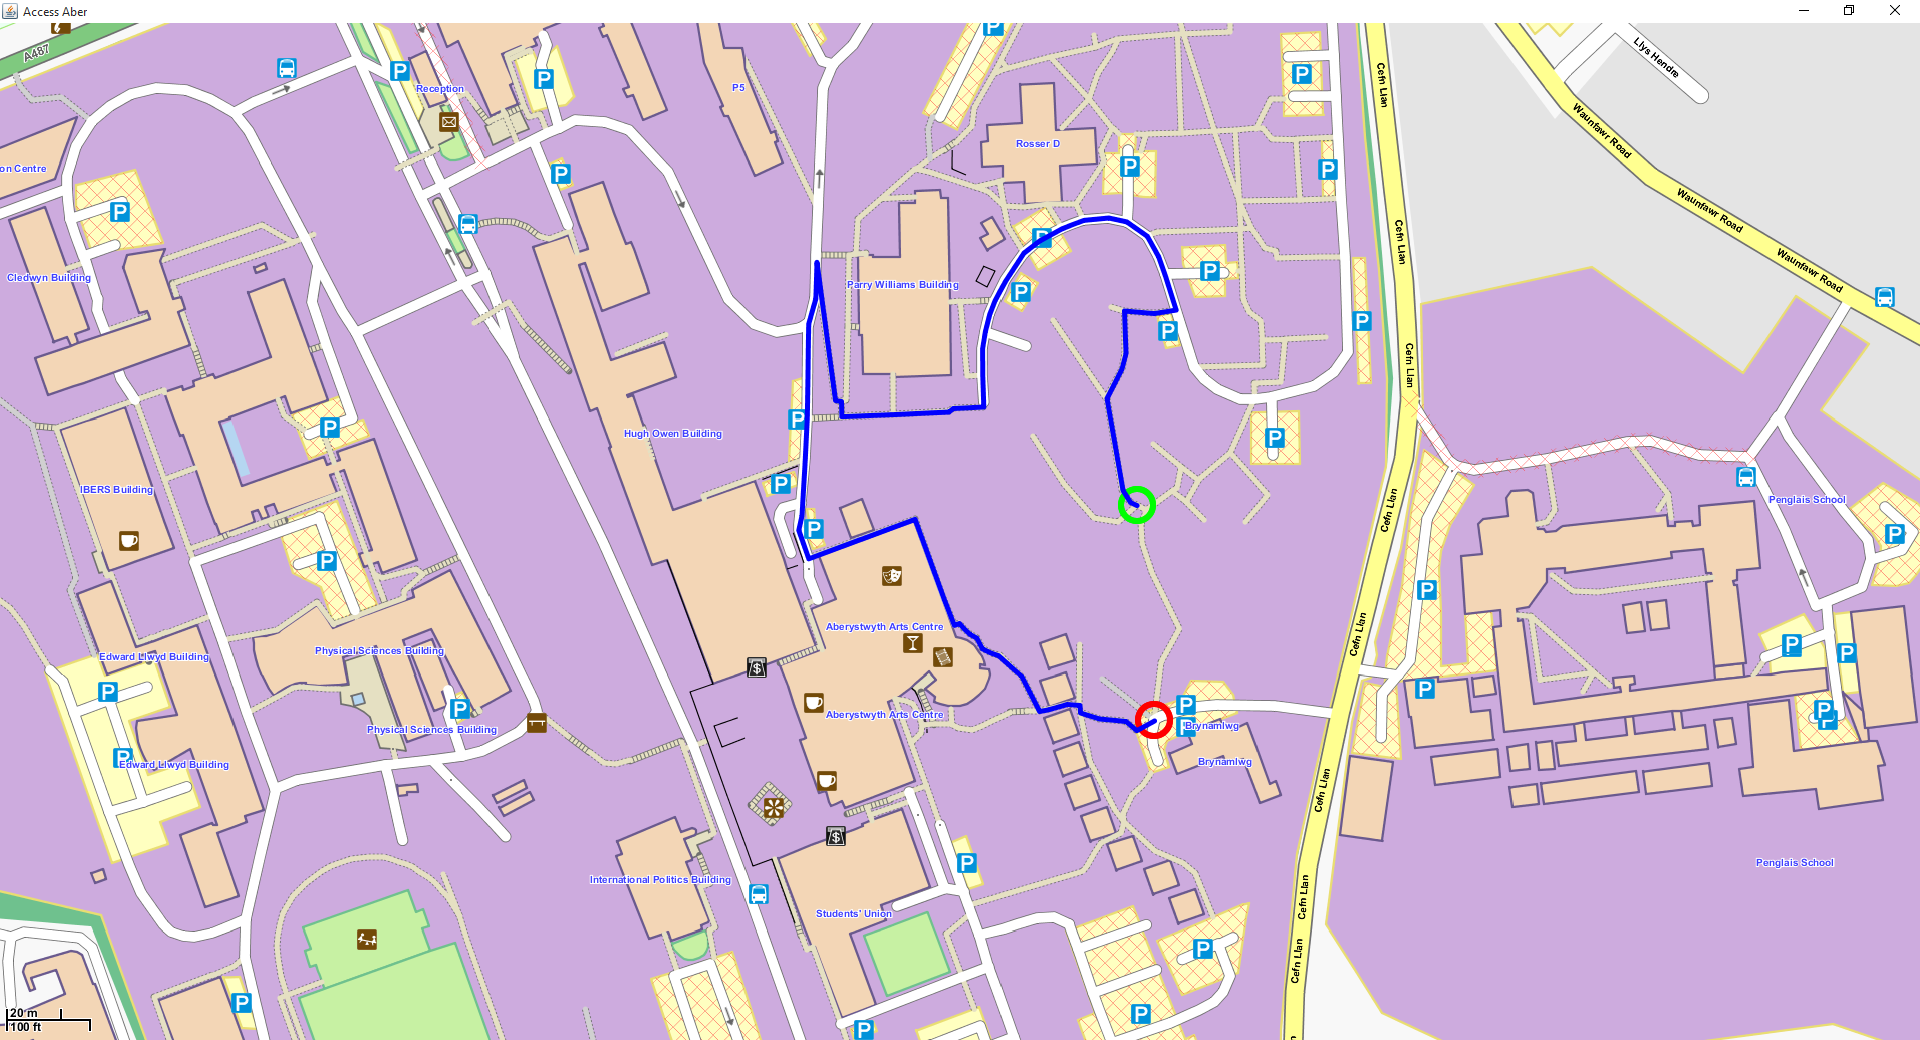
\includegraphics[keepaspectratio, width=\columnwidth]{Images/AStar_Missing_Node-data}}
\end{figure}

\begin{figure}
	\centering
	\caption{Algorithms avoid stairs}
	\label{fig:avoidStairs}
	\frame{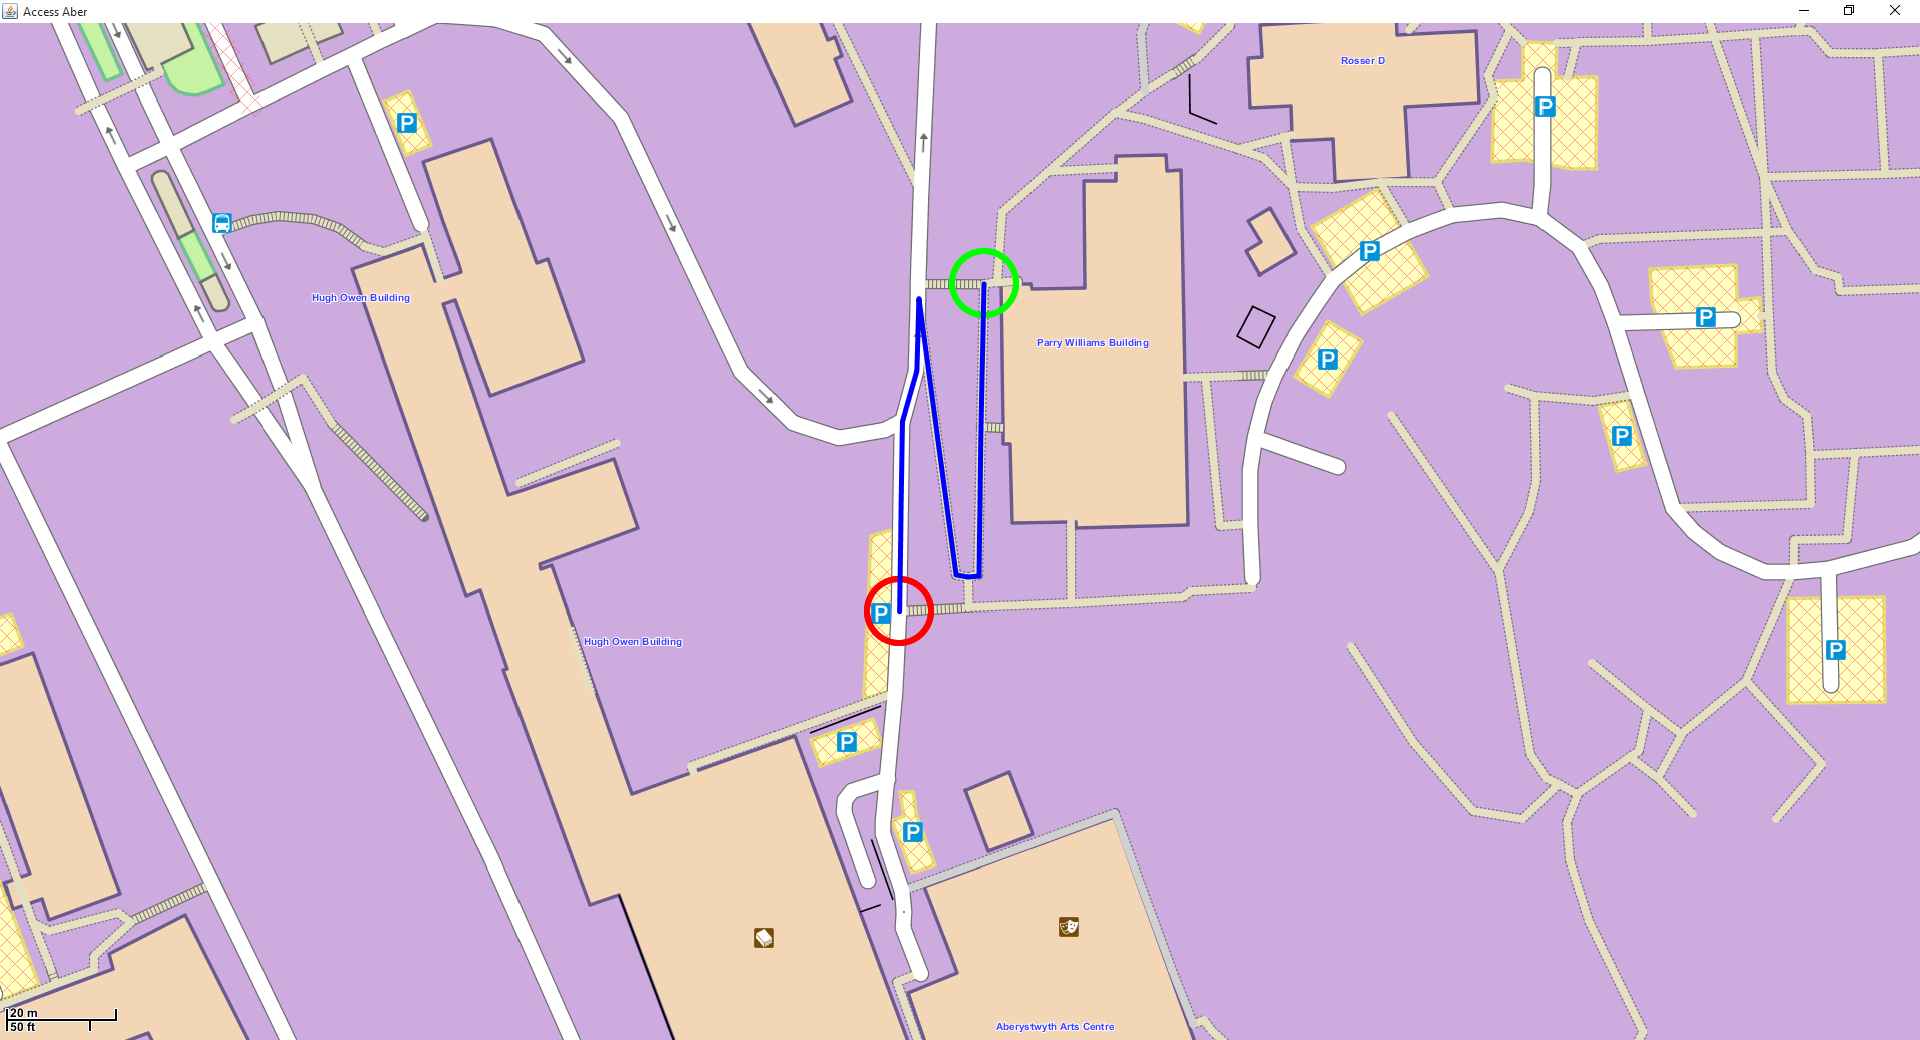
\includegraphics[keepaspectratio, width=\columnwidth]{Images/AStar_Avoids_stairs}}
\end{figure}
\begin{figure}
	\centering
	\caption{Algorithms avoid stairs 2}
	\label{fig:avoidStairs2}
	\frame{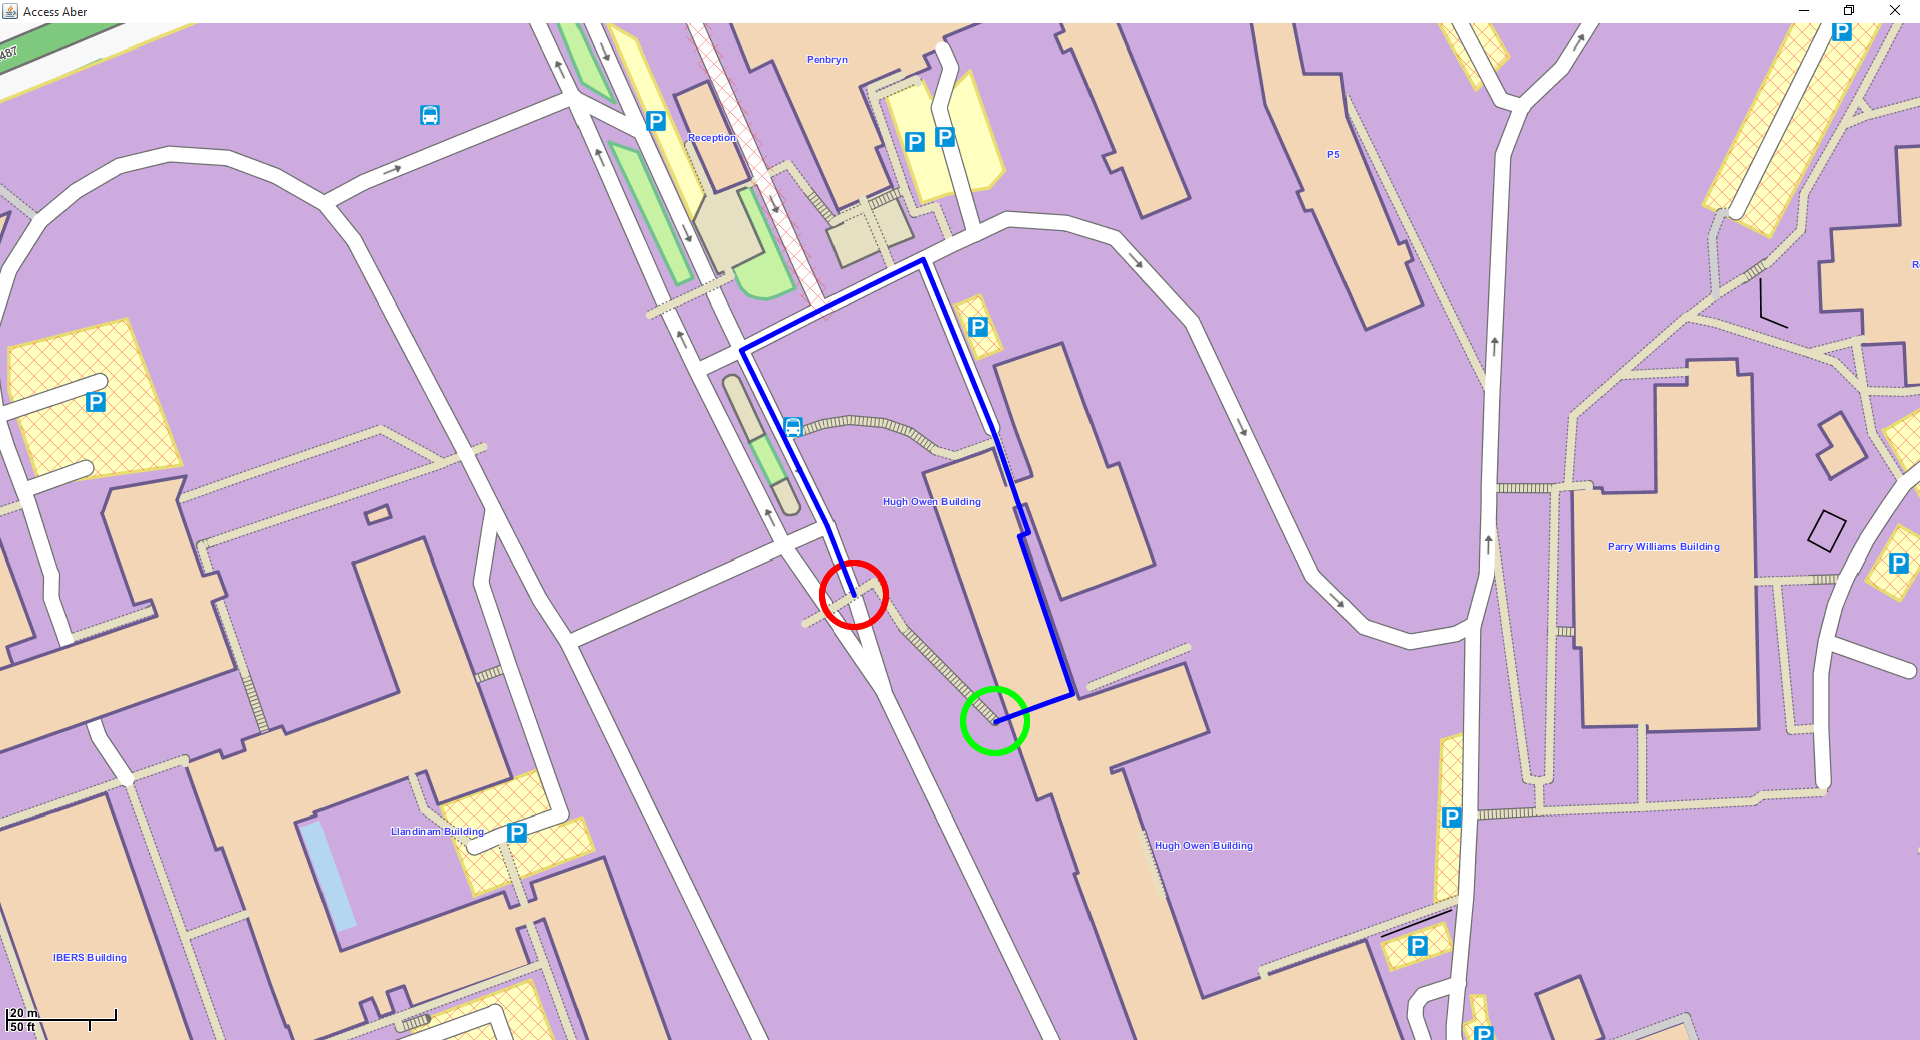
\includegraphics[keepaspectratio, width=\columnwidth]{Images/AStar_Avoids_stairs2}}
\end{figure}

\section{Map}
\textbf{NOTES: - DELETE THIS -}
\begin{itemize}
	\item Map-API from Mapsforge \cite{Mapsforge}. GraphHopper considered; they also use Mapsforge.
\end{itemize}




\section{Fulfilment of requirements}
\textbf{NOTES: - DELETE THIS -}
\begin{itemize}
	\item Storage of OSM-data in separate Arrays for Nodes and Ways.
	\item OpenStreetMap database not updated with new and/or more accurate information.
	\item Good routing-algorithm found; A* guarantees optimality and completeness. Other algorithms are able to use less memory and find routes faster, but A* works fine on a small area like the Penglais campus of Aberystwyth University.
	\item Created filters able to easily exclude many Nodes/Ways from the search. Very easy to add and remove labels in the filters. Filters made for wheelchair-users only.
	\item No localisation (eg. GPS) implemented, but added functionality to find the Node closest to some coordinates and set it as the start/goal position, thus making it relatively easy to use localisation to set the user's position in the future. The coordinates need to use the same coordinate-system as the OSM-data though.
\end{itemize}

